\documentclass[border=10pt]{standalone}
\usepackage{pgfplots}
\pgfplotsset{compat=1.18}
\begin{document}
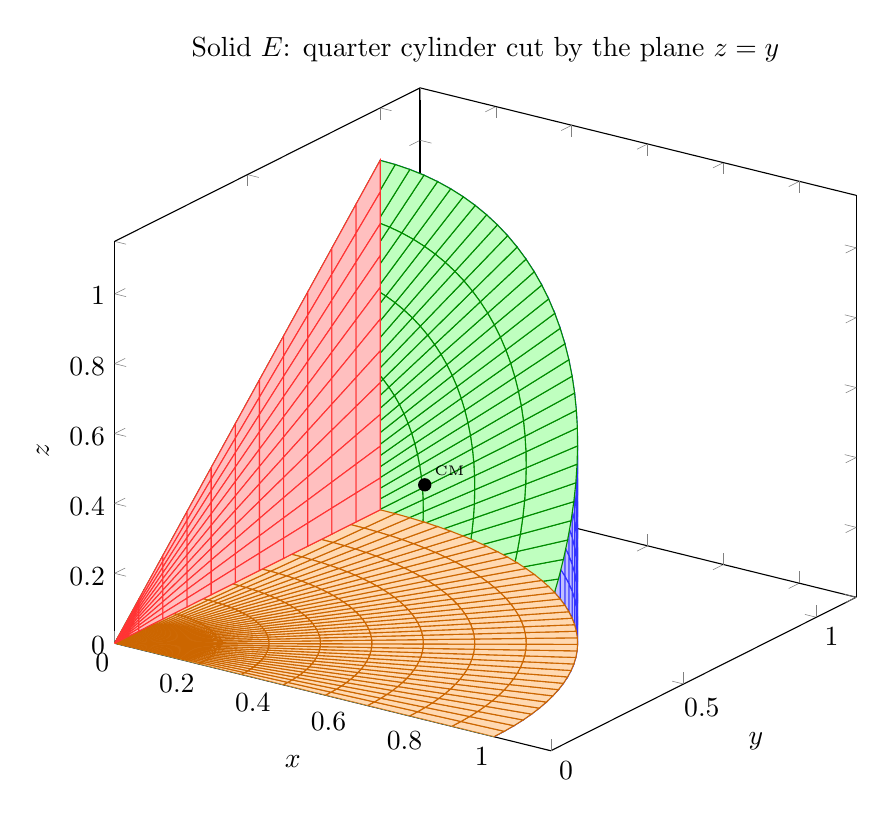
\begin{tikzpicture}
\begin{axis}[
    view={35}{25},
    xlabel=$x$, ylabel=$y$, zlabel=$z$,
    trig format plots=rad,
    xmin=0,xmax=1.15,ymin=0,ymax=1.15,zmin=0,zmax=1.15,
    width=11cm,height=10cm,
    title={Solid $E$: quarter cylinder cut by the plane $z=y$}]
% cylinder curved side  (blue)
\addplot3[surf, shader=faceted, fill=blue!25, faceted color=blue!80,
          domain=0:1.5708, y domain=0:1, samples=40, samples y=10]
  ({cos(x)}, {sin(x)}, {y*sin(x)});
% top plane z=y  (green)
\addplot3[surf, shader=faceted, fill=green!25, faceted color=green!55!black,
          domain=0:1.5708, y domain=0:1, samples=40, samples y=10]
  ({y*cos(x)}, {y*sin(x)}, {y*sin(x)});
% bottom disk z=0  (orange)
\addplot3[surf, shader=faceted, fill=orange!30, faceted color=orange!80!black,
          domain=0:1.5708, y domain=0:1, samples=40, samples y=10]
  ({y*cos(x)}, {y*sin(x)}, {0});
% side x=0 triangle  (red)
\addplot3[surf, shader=faceted, fill=red!25, faceted color=red!80,
          domain=0:1, y domain=0:1, samples=12]
  ({0}, {x}, {x*y});
% center of mass
\addplot3[only marks, mark=*, mark size=2.2pt, color=black]
  coordinates {(0.387,0.615,0.322)};
\node at (axis cs:0.387,0.615,0.322) [above right,font=\tiny]{CM};
\end{axis}
\end{tikzpicture}
\end{document}